\documentclass[mcs]{scsthesis}
\usepackage{url}
\usepackage{amsmath}
\usepackage{graphicx}
\title {Biased Nearest Neighbour Search}
\author {Daniel Minor}
\thesissupervisor {Patrick Morin}
\director {Douglas Howe}
\begin{document}

\beforepreface

\prefacesection

\chapter*{Abstract}

TODO:

\chapter*{Acknowledgements}

TODO:

\afterpreface

\chapter{Introduction}

\section{Problem Statement}

We investigate the utility of distribution sensitive data structures for
geometric search problems in practice.  A distribution sensitive data structure
makes use of a priori knowledge of the probability distribution of queries in
order to answer common queries more quickly, giving an expected runtime which
is of the order of the entropy, or amount of randomness, present in the query
distribution.

Recently, two groups of researchers \cite{chan} \cite{oddson} have proposed a
theoretical framework for a distribution sensitive data structure which can be
applied to a variety of geometrical search problems which seems as though it
may be of practical as well as theoretical interest.  Following \cite{oddson},
we will call this data structure the Odds-on tree.

The geometrical search problem used to investigate these results is nearest
neighbour search.  The nearest neigbhour search problem is: given a query
point, a set of other points, and a metric, return the closest point to the
query point in the set of the points under the specified metric.  Two related
problems are k-nearest neighbours search, where the k closest points to the
query point are returned, and approximate nearest neighbour search, where the
points returned are closest only up to a specified tolerance.  These problems
are of considerable practical interest, with applications in GIS, computer
graphics, computer vision, signal processing and machine learning.

In this thesis we examine Odds-on trees through the lens of algorithm
engineering.  Our goal is to study the design decisions and implementation 
techniques required to derive a practical data structure from the theoretical
results about Odds-on trees.  This involves both development work and
extensive experimentation to establish correctness and performance under a
variety of query distributions, both derived from probability distributions,
and from some applications of practical interest.  

\section{Definitions}

TODO:

\section{Results Summary}

TODO:

\section{Organization of the Thesis}

The remainder of the thesis is organized as follows: Chapter 2 summarizes
previous work for biased search, distribution sensitive data structures and
nearest neighbour search.  Chapter 3 describes the design and implementation of
the Odds-on Tree, including an description of alternative designs which were
explored.  Chapter 4 gives details on the experiemntation performed and results
obtained, and Chapter 5 summarizes the results and discusses potential 
future work.

\chapter{Previous Work}

\section{Biased Search}

\subsection{Biased Search Trees}

Biased search trees are a natural generalization of balancing a binary search
tree where rather than assuming each result is equally likely, a probability
distribution is given for the results, allowing the tree to be balanced such
that at each node it is equally likely that the left or right child will be
followed.  The overall expected running time can then be stated in terms of the
entropy of the probability distribution of the queries.

Early work on biased search trees is described in Knuth \cite{knuth} where
the static case (i.e. no deletions and insertions) is considered.  An \(O(n^2)\)
dynamic programming algorithm is presented which constructs an optimum static
search tree for a set of weights.

Biased search trees allowing insertions and deletions based upon 2 - 4 and
red-black trees were described by Bent, Sleator and Tarjan \cite{bst}.  The
data structures are complex and do not appear to have been implemented.
Feigenbaum and Tarjan describe somewhat simpler data structures \cite{bst2}. A
much simpler implementation of biased search based upon randomized search trees
was developed by Aragon and Seidel \cite{treap}, and a biased version of skip
lists \cite{skiplist} was presented in \cite{bsl2}.

An alternative approach to biased search is to use data structures which
modify themselves in response to queries.  In this case, rather than specifying
the probabilities in advance, the data structure will change itself to match
the query distribution.  Splaytrees \cite{splaytree}, which were invented by
Sleator and Tarjan, are a self-modifying binary search tree which have
received considerable attention, both theoretical and experimental due to the
dynamic optimality conjecture, which states that splaytrees are within a
constant factor of optimal for any sequence of queries, without needing to
know the queries in advance.

Most experimental work with biased search has focused on comparing splaytrees
with traditional approaches like 2 - 4 trees and red-black trees.

TODO: give some references on previous experimental work with biased search.

\subsection{Distribution Sensitive Data Structures}

A distribution sensitive data structure has a running time which is a multiple 
of the entropy of the query distribution.  This is similar to biased search
trees, where the running time is given in terms of the entropy of the query
results, but provides a better framework for examining geometric search
problems.

TODO: Explain why better for geometric search.

TODO: Refer to at least Biased Range Trees paper, some results in distribution
sensitive point location.

\subsection{Instance Optimality}

An instance optimal data structure \cite{chan} has a running time which is
within a constant factor of any data structure for any instance of the problem.

TODO: Explain why this gives equivalent results to distribution sensitive data
structures.

\section{Nearest Neighbour Search}

TODO: Knuth on post-office query, Bentley's quadtrees and kd-trees.  Fast
vector quantization paper, ANN.  Metric trees, Locality sensitive hashing

\chapter{Implementation}


In both \cite{oddson} and \cite{chan} the data structure is based upon
Matousek's partition trees \cite{matousek}.  Partition trees have nice
theoretical properties, but are not practical to implement.

TODO: Explain why they are not practical.

This chapter gives alternative implementations based upon kd-trees and
quadtrees, two commonly used data structures for point location and nearest
neighbour search.  We begin with a description of the partition tree based
implementation, as ideas from it are used in both the kd-tree and quadtree
based implementations.

\section{Odds-on Trees}

TODO: Description of partition tree based Odds-on tree.


\section{Kd-tree Implementation}

The backup

The initial implementation of Odds-on Trees closely followed the description of
the data structure given in \cite{oddson} but used kd-trees rather than
partition trees.

\section{Kd-tree Based Odds-on Tree}

TODO: Brief overview of kd-tree data structure and how it was implemented.  This
is also the implementation of the back up oracle for both implementations and the
baseline for experimentation. 

\section{Construction algorithm}

\section{Query algorithm}

\section{Quadtree Based Odds-on Tree}

\subsection{Z-Order and Quadtrees}

TODO: Quick overview of Z-Order, outline Chan's algorithm, and the extension to
floating point numbers.

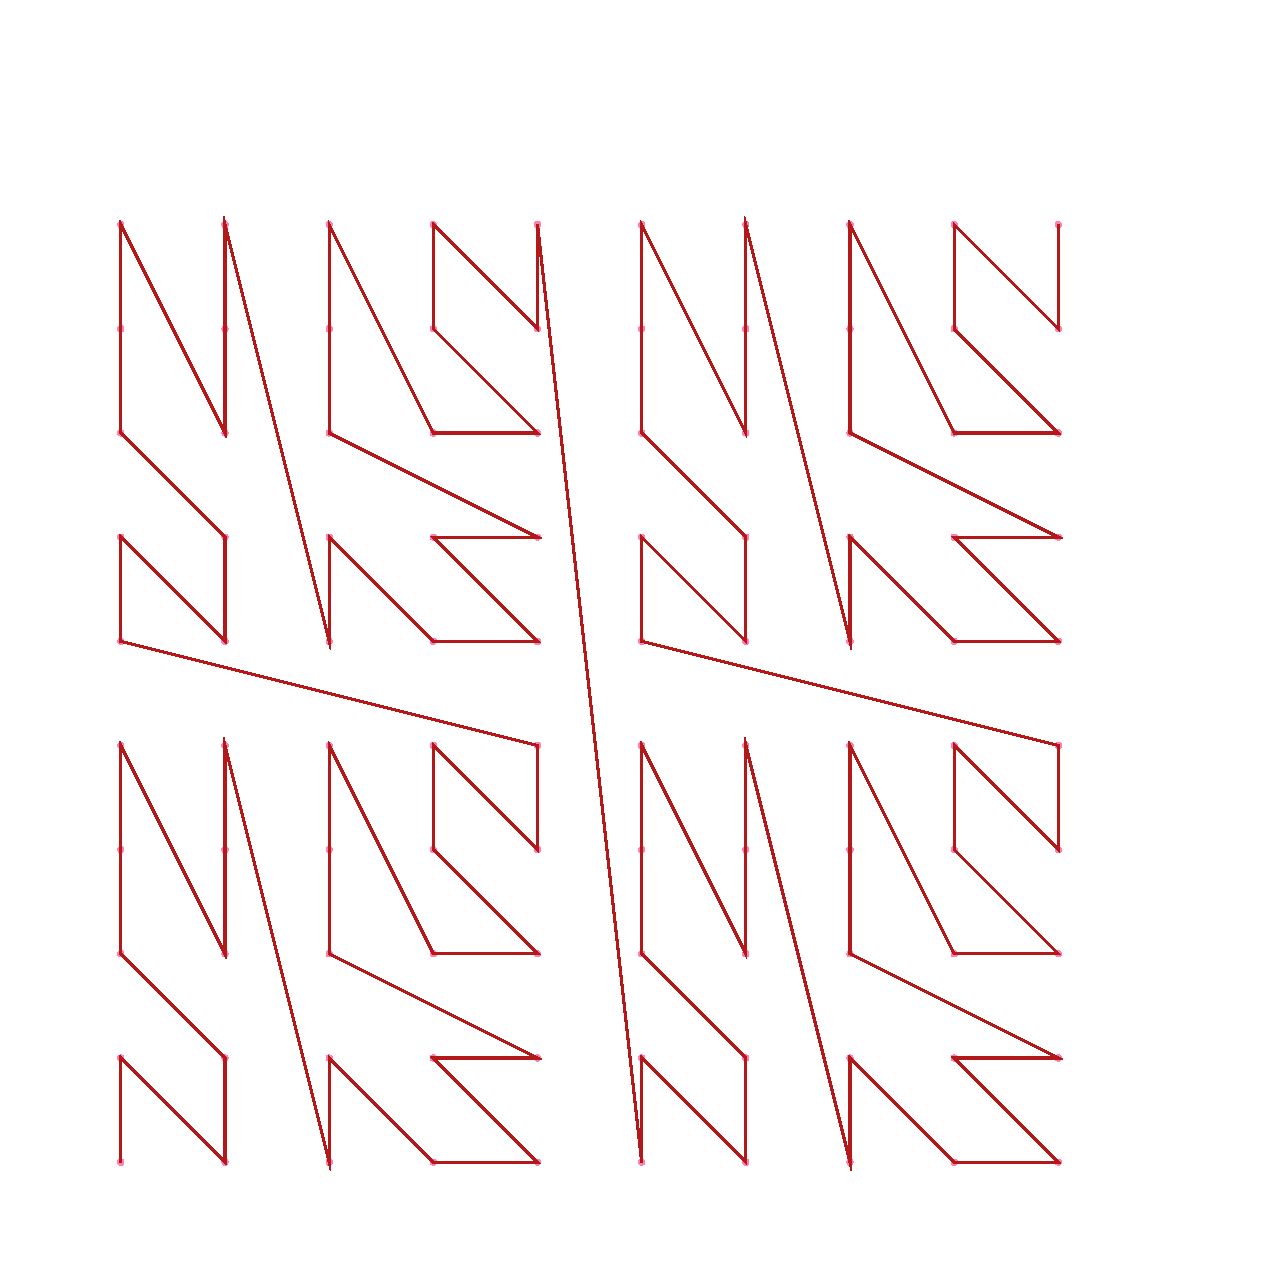
\includegraphics[scale=0.4]{diagrams/zorder.eps}

\subsection{Construction algorithm}

TODO: Outline how quadtree is built once points are sorted into z-order.

\section{Performance Tuning}

TODO: Do some profiling to see if there are any spots which can be optimized. 
TODO: Do experimentation to determine appropriate sample size.
TODO: Do experimentation to determine whether or not it is best to sort by NN
      then by z-order or not.

\chapter{Experimental Results}

\section{Experiment Design}

The experimental hypothesis is that the odds-on tree provides better k-nn
performance than a kd-tree implementation in cases where the entropy of the
query set is sufficiently low.

The implementations were tested with both synthetic data and data derived
from applications of nearest neighbour search.

Three separate sets of data are required for each experimental run.  The first
is the point set which is the subject of the searches, the second is the point
set which is used as samples to build the odds-on tree, and the third is the
point set used to query the odds-on tree and the kd-tree.  For all of the
synthetic data sets,  second and third data sets were derived from the same
distribution.

TODO: briefly describe distributions used to generate points: uniform, gaussian,
mixture of gaussians.


\section{Measuring Performance}

\subsection{Benchmark Platform}

An Intel Core I5 laptop was used as the benchmark platform.

TODO: Possibly also run experiments on an ARM processor?

\subsection{Performance Metrics}

The primary performance metric is running time.  For each experiment
configuration, 1000000 queries were performed and the elapsed system clock
time was recorded.

In addition to running time, data was collected on the cache miss rate for the
odds-on tree, as well as the number of nodes visited in both the cache and the
back up tree.

Since cache utilization can have a major impact on running time, the Valgrind
\cite{valgrind} cachegrind utility was used to simulate the cache performance
of the implementation, and data was collected on L1 and L2 cache miss rates.

\section{Results}

TODO: one section for each experimental configuration.

\chapter{Conclusion}

\section{Summary}

TODO:

\section{Future Work}

TODO:

\begin{thebibliography}{5}

\bibitem{treap}
Aragon, C. R.,  Seidel, R. (1996) Randomized Search Trees.
In Algorithmica, Vol. 16, Number 4/5, pp. 464 – 497

\bibitem{bsl}
Bagchi,A. Buchsbaum, A. L., Goodrich, M. T. (2005) Biased Skip Lists.
In Algorithmica Vol. 42, pp. 31 – 48
 
\bibitem{splaytree}
Sleator, D. D., Tarjan, R. E. (1985) Self-adjusting binary search trees.
In Journal of the ACM, 32, pp. 652 – 686

\bibitem{knuth}
Knuth, D. E. (1998) The Art of Computer Programming, Second Edition,
Volume 3, Sorting and Searching.  Addison-Wesley, Reading, Massachusetts, USA.

\bibitem{bst}
Bent, S. W., Sleator, D. D., Tarjan, R. E. (1984) Biased Search Trees,
In SIAM Journal on Computing, Volume 14, pp. 545 - 568

\bibitem{bst2}
Feigenbaum, J., Tarjan, R. E. (1983) Two New Kinds of Biased Search Tree,
In Bell Systems Technical Journal, Vol. 62, No. 10, pp. 3139 - 3158

\bibitem{skiplist}
Pugh, W. (1990) Skip Lists: A Probabilistic Alternative to Balanced Trees.
In Communications of the ACM, 33(6), pp. 668 – 676

\bibitem{bsl2}
Ergun, F., Sahinalp, S. C., Sharp, J., Sinha, R. K. (2001) Biased Skip Lists
for Highly Skewed Access Patterns, Proceedings of ALENEX 2001, Lecture Notes in
Computer Science, Volume 2153, 216-229

\bibitem{satp}
Williams, H. E., Zobel, J., Heinz, S. (2001) Self-Adjusting Trees in Practice
for Large Text Collections, In Software - Practice and Experience,
Volume 31, pp. 925 - 939

\bibitem{valgrind}
Nethercote, N., Seward, J. (2007) Valgrind: A Framework for Heavyweight Dynamic
Binary Instrumentation.  Proceedings of ACM SIGPLAN 2007 Conference on
Programming Language Design and Implementation (PLDI 2007),
San Diego, California, USA

\end{thebibliography}

\end{document}
